\pagestyle{fancy}
\fancyhf{}
\rhead{ Chapitre 4 : Réalisation}
\rfoot{Page \thepage}
\lfoot{\includegraphics[scale=0.1]{figures/ooredoo.png}\\[0.1cm]}

\chapter{ Réalisation }
\newpage
\section{Introduction}
Après avoir élaboré la conception de notre application, nous abordons dans ce chapitre la dernière branche de la méthodologie suivie, qui a pour objectif d'exposer la phase de réalisation.

La phase de réalisation est considérée comme étant la concrétisation finale de toute la méthode de conception. Nous menons tout d’abord notre choix de l’environnement de travail, ensuite nous présenterons la mise en place pratique de notre travail. Enfin, nous clôturons ce chapitre par la présentation des interfaces homme-machine des tableaux de bord créés et du chatbot.

\section{Environnement matériel et logiciel}

Pour la réalisation de cette solution, nous avons eu recours à plusieurs moyens matériels et logiciels :

\subsection{Environnement matériel}

L’environnement matériel sur lequel nous avons travaillé est constitué de mon PC personnel, caractérisé par :

\begin{itemize}
    \item Système d’exploitation : Windows 11
    \item Processeur : AMD Ryzen 5 5600H
    \item RAM : 32 Go
    \item Disque dur : 512 Go SSD M.2 NVMe
    \item Carte graphique : NVIDIA GeForce RTX 3050
\end{itemize}

\subsection{Environnement logiciel}

Après avoir présenté les moyens matériels, nous abordons dans cette partie l’environnement logiciel utilisé pour le développement de l’application :

\begin{itemize}
    \item \textbf{Talend} : Outil ETL pour l'extraction, la transformation et le chargement des données.
    \item \textbf{Power BI} : Logiciel décisionnel pour la création des tableaux de bord dynamiques.
    \item \textbf{XAMPP} : Serveur local incluant Apache, MySQL, et PHP.
    \item \textbf{Frameworks} : Laravel pour le backend et Nuxt.js pour le frontend.
\end{itemize}

\section{Réalisation de la phase ETL}

Dans cet axe, nous allons décrire les étapes de mise en œuvre du processus ETL pour migrer les données Excel historiques vers la base de données MySQL.
\subsection{Composants Talend utilisés}

Les outils utilisés pour la phase ETL incluent :

\begin{itemize}
    \item \textbf{TFileInputExcel} : Composant permettant de lire les données à partir de fichiers Excel. Il lit les données de chaque feuille spécifiée via l’option "Liste des feuilles" et les intègre dans les flux de données Talend. Si les feuilles ont la même structure, un seul composant suffit ; sinon, plusieurs composants sont nécessaires pour gérer des structures différentes (ex. "Feuille\_A" et "Feuille\_B").
    
    \item \textbf{TMap} : Composant central pour le mappage et la transformation des données. Il permet de gérer les colonnes, d’effectuer des conversions de types, des calculs, et de gérer plusieurs flux en entrée ou en sortie.
    
    \item \textbf{tDBOutput} : Composant utilisé pour charger les données transformées dans une base MySQL. Il offre des options de connexion, de mappage des colonnes, ainsi que de gestion des erreurs.
    
    \item \textbf{tFilterRow} : Utilisé pour filtrer les données selon des conditions définies (ex. suppression des lignes avec des valeurs nulles), avec la possibilité d’utiliser des opérateurs logiques (AND, OR).
    
    \item \textbf{tJavaRow} : Permet d’exécuter du code Java personnalisé pour chaque ligne, par exemple pour la génération d’identifiants uniques.
\end{itemize}
\vspace{0.5cm}
\begin{table}[h!]
    \centering
    \begin{tabular}{|l|p{10cm}|}
        \hline
        \textbf{Composant} & \textbf{Description} \\
        \hline
        TFileInputExcel & Lit les données Excel avec option pour spécifier les feuilles. \\
        \hline
        TMap & Mappage et transformation des données (jointures, conversions). \\
        \hline
        tDBOutput & Charge les données dans MySQL avec gestion des erreurs. \\
        \hline
        tFilterRow & Filtre les données selon des conditions définies. \\
        \hline
        tJavaRow & Exécute du code Java personnalisé (ex. génération d'IDs). \\
        \hline
    \end{tabular}
    \caption{Composants Talend utilisés}
    \label{tab:talend_components}
\end{table}

\subsection{Alimentation de la base de données}
Cette section décrit la méthodologie adoptée pour importer les données historiques contenues dans les fichiers Excel EBDS, tels que \\\textit{Expression\_de\_Besoin\_Detaille\_monitoring\_Service\_MyOoredoo\_Support\_ASE\_VAS.XLSX} , \\ dans la base de données MySQL. L’objectif est de transformer et de charger les données de supervision (serveurs, URLs, processus, etc.) de manière structurée, en utilisant Talend pour assurer une migration fiable et performante.

Étape par étape pour importer les fichiers Excel EBDS, tels que \\\textit{Expression\_de\_Besoin\_Detaille\_monitoring\_Service\_MyOoredoo\_Support\_ASE\_VAS.XLSX} , dans MySQL :

\begin{itemize}
    \item \textbf{Étape 1 : Configuration du TFileInputExcel}  
      Utilisez le composant TFileInputExcel pour lire les données des fichiers Excel EBDS, en spécifiant les feuilles à lire (ex. onglets Serveurs, Process, Url). Cette étape nécessite de configurer le chemin du fichier, de sélectionner les feuilles pertinentes (par exemple, "Serveurs" pour les données d'hôtes), et de définir le schéma des colonnes (ex. `N° Réf.`, `Réf.`, `État`). Assurez-vous de gérer les en-têtes et de spécifier l'encodage (UTF-8) pour éviter les problèmes de caractères. Une capture d’écran illustre la configuration du composant avec les paramètres de feuille et de schéma.
      
      \begin{figure}[h]
          \centering
          \frame{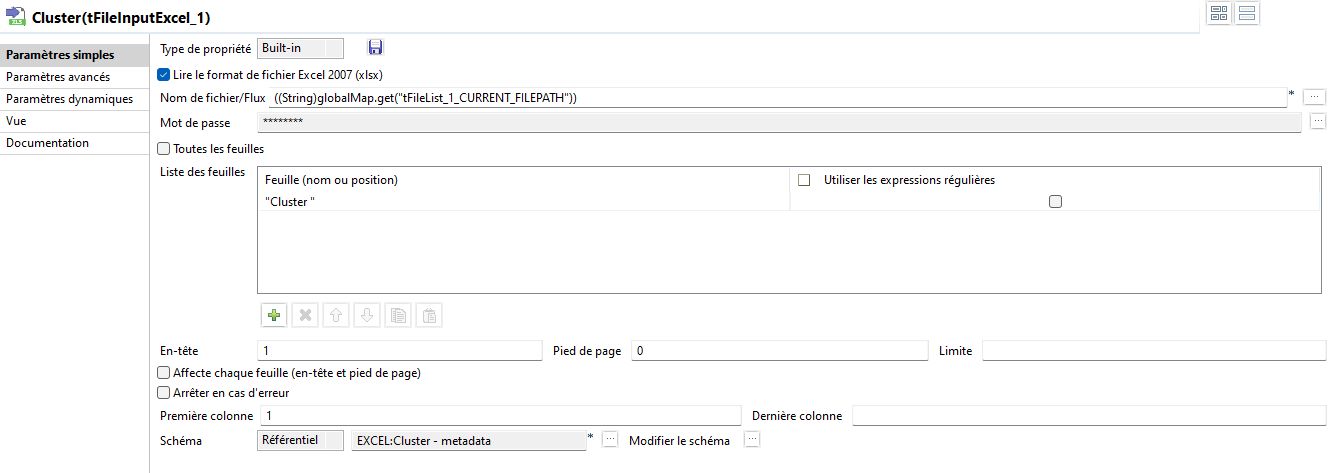
\includegraphics[width=0.8\textwidth,height=0.4\textwidth]{figures/chap4 fig/etl_step1_tfileinputexcel.png}}
          \caption{Configuration de TFileInputExcel}
          \label{fig:etl_step1}
      \end{figure}
      
    \item \textbf{Étape 2 : Utilisation de tFilterRow}  
      Appliquez le composant tFilterRow pour filtrer les colonnes vides ou non pertinentes avec des expressions conditionnelles (ex. `row1.N° Réf. != null && row1.État != ''`). Cette étape élimine les lignes incomplètes, comme celles sans `Plateforme` ou `Hostname`, et garantit que seules les données valides (ex. statuts "Nouveau" ou "Modifié") sont conservées. Une gestion rigoureuse des filtres permet de réduire les erreurs lors de la transformation. Une capture montre l’interface de filtrage avec une expression d’exemple.
      
      \begin{figure}[h]
          \centering
          \frame{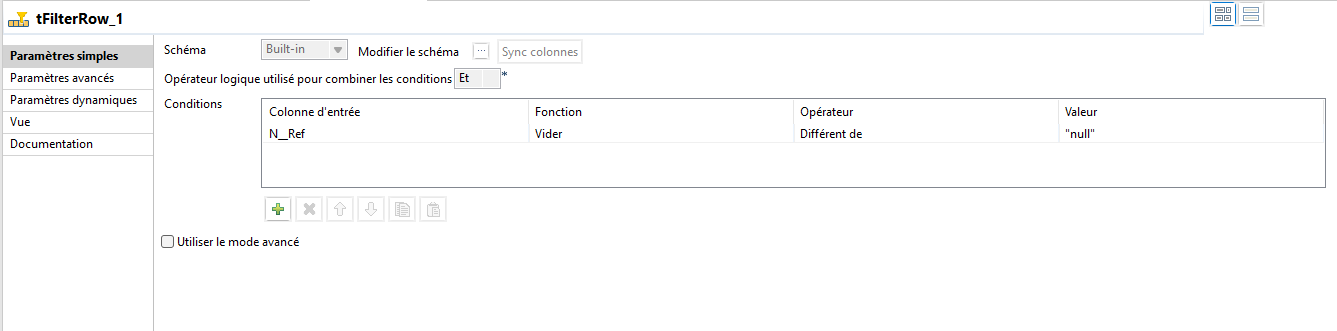
\includegraphics[width=0.8\textwidth,height=0.4\textwidth]{figures/chap4 fig/etl_step2_tfilterrow.png}}
          \caption{Configuration de tFilterRow}
          \label{fig:etl_step2}
      \end{figure}
      \newpa
   \item \textbf{Étape 3 : Génération de l'ID}  
Utilisez le composant \texttt{tJavaRow} pour générer un ID unique par ligne, par exemple en combinant le nom du fichier (ex. \texttt{"MyOoredoo"}) et un compteur incrémental (ex. \texttt{"MyOoredoo\_001"}).

\vspace{2mm}

Cet ID est stocké dans une colonne supplémentaire, comme \texttt{custom\_id}, pour assurer la traçabilité des enregistrements migrés. Cette étape est cruciale pour éviter les doublons lors de l’intégration avec la table \texttt{demandes}. Une capture illustre le code Java personnalisé dans \texttt{tJavaRow}.
      
      \begin{figure}[h]
          \centering
          \frame{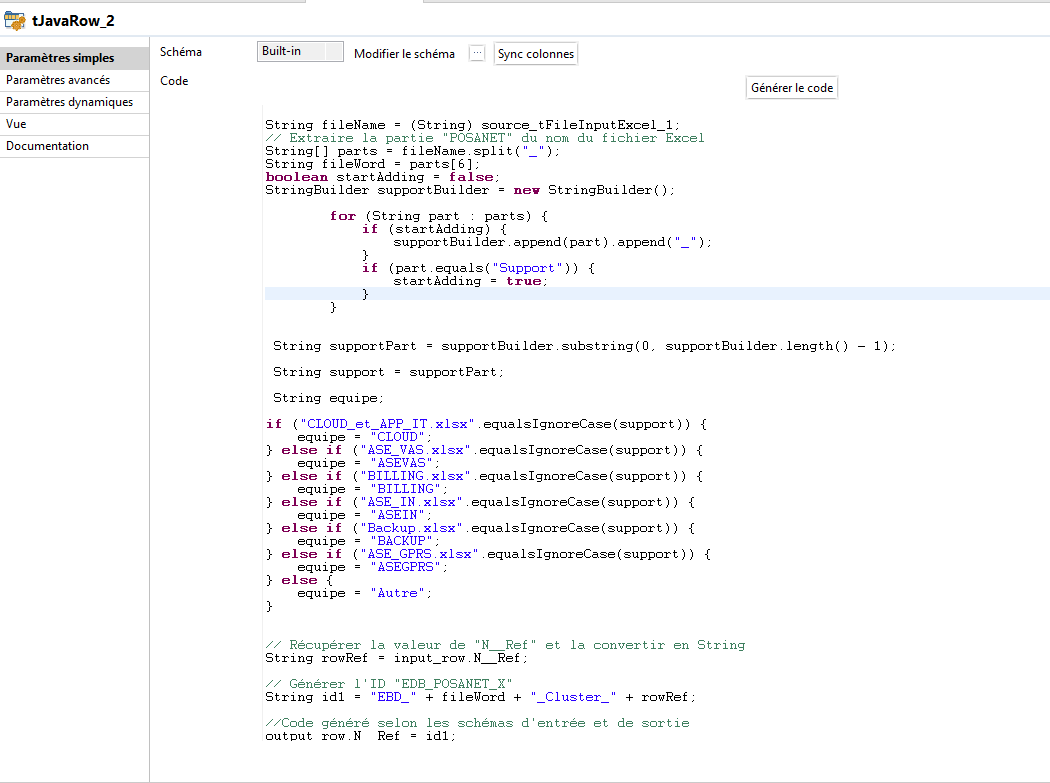
\includegraphics[width=0.8\textwidth,height=0.4\textwidth]{figures/chap4 fig/etl_step3_tjavarow.png}}
          \caption{Configuration de tJavaRow pour la génération d’ID}
          \label{fig:etl_step3}
      \end{figure}
      
    \item \textbf{Étape 4 : Utilisation de tMap}  
      Employez le composant tMap pour mapper et transformer les données, en connectant TFileInputExcel et tJavaRow. Cette étape inclut la conversion de types (ex. texte en date pour `created\_at`), l’ajout de colonnes dérivées (ex. `criticite\_id` basé sur des règles), et la gestion des jointures implicites avec d’autres tables (ex. `serviceplatfom\_id`). Une validation des données transformées est effectuée pour s’aligner sur le schéma MySQL. Une capture montre la vue de mappage avec les transformations appliquées.
      
      \begin{figure}[h]
          \centering
          \frame{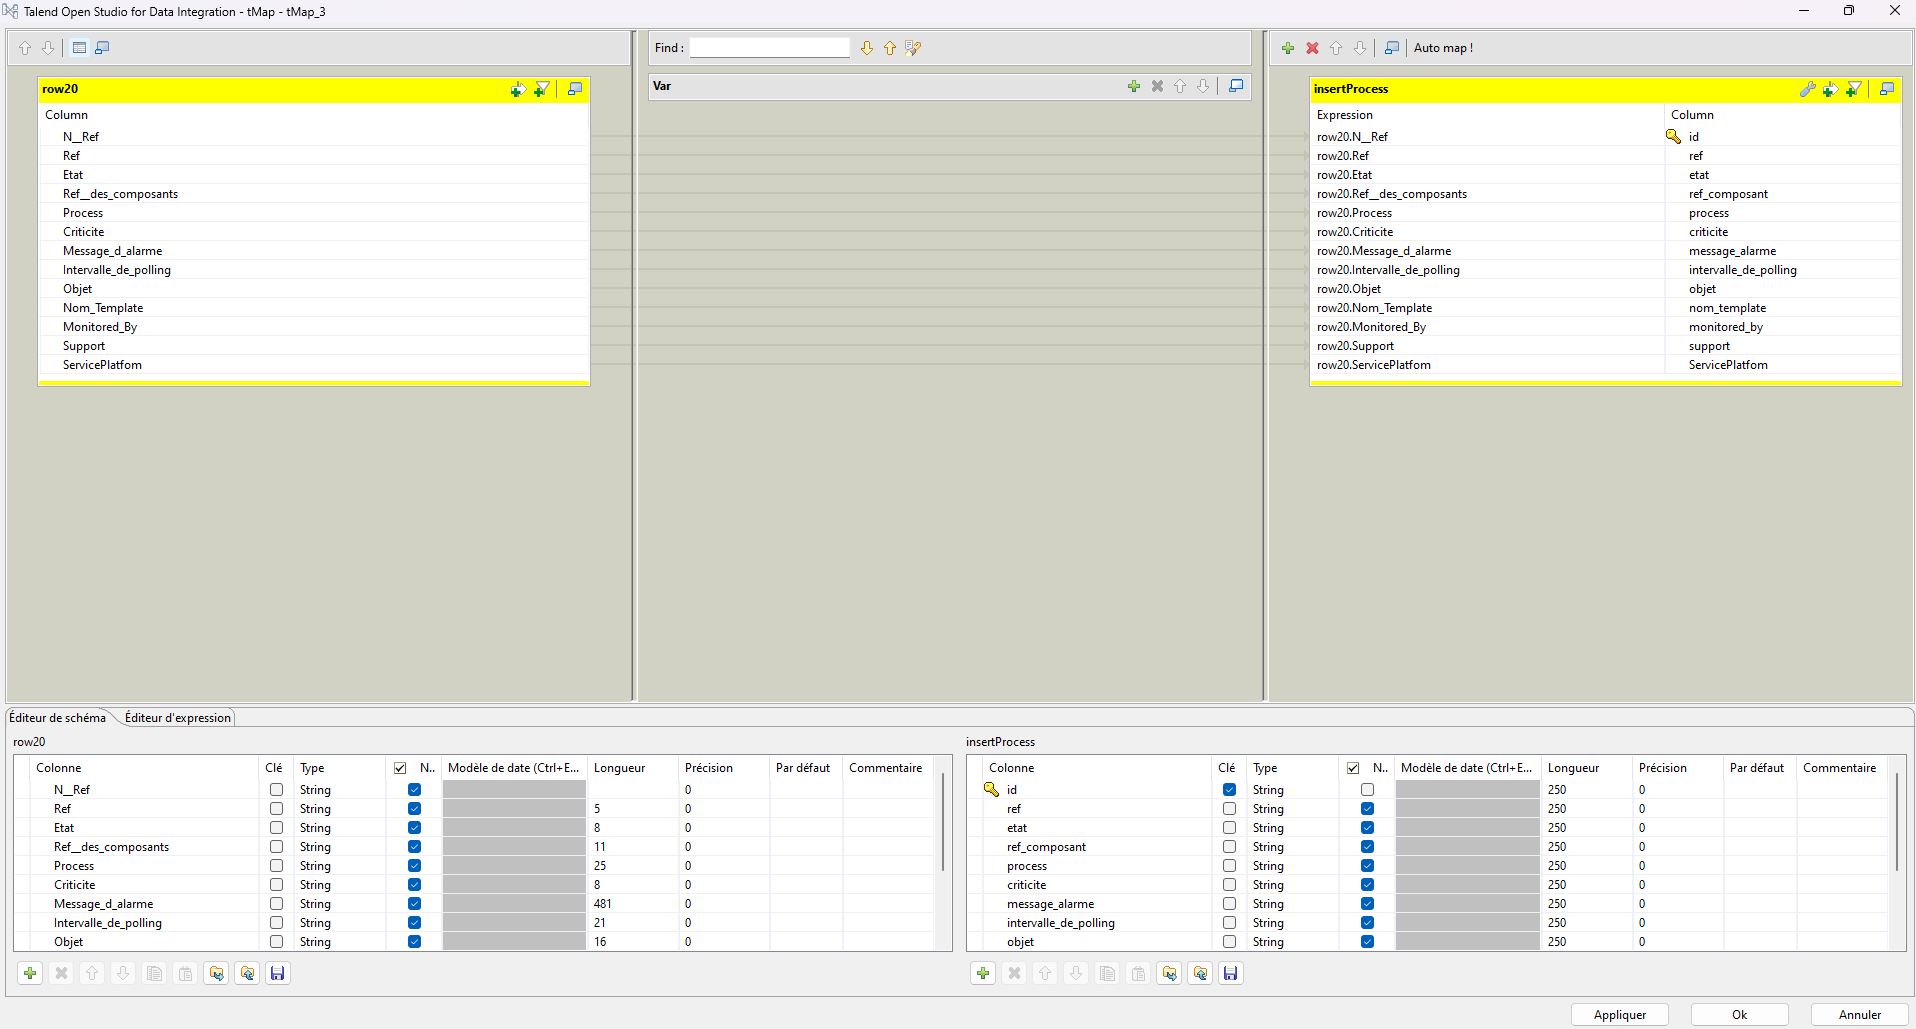
\includegraphics[width=0.8\textwidth,height=0.4\textwidth]{figures/chap4 fig/etl_step4_tmap.png}}
          \caption{Configuration de tMap}
          \label{fig:etl_step4}
      \end{figure}
      
    \item \textbf{Étape 5 : Chargement dans la base de données}  
      Utilisez le composant tDBOutput pour insérer les données transformées dans MySQL, en mappant les colonnes au schéma cible (ex. `demandes`, `serveurs`, `url`). Configurez les options d’insertion (insert or update) pour gérer les doublons et activez les journaux d’erreurs pour dépanner les échecs. Cette étape optimise les performances en utilisant des lots (batch size) et valide l’intégrité référentielle avec les clés étrangères (ex. `user\_id`). Une capture illustre la configuration de tDBOutput avec le mappage des colonnes.
      
      \begin{figure}[h]
          \centering
          \frame{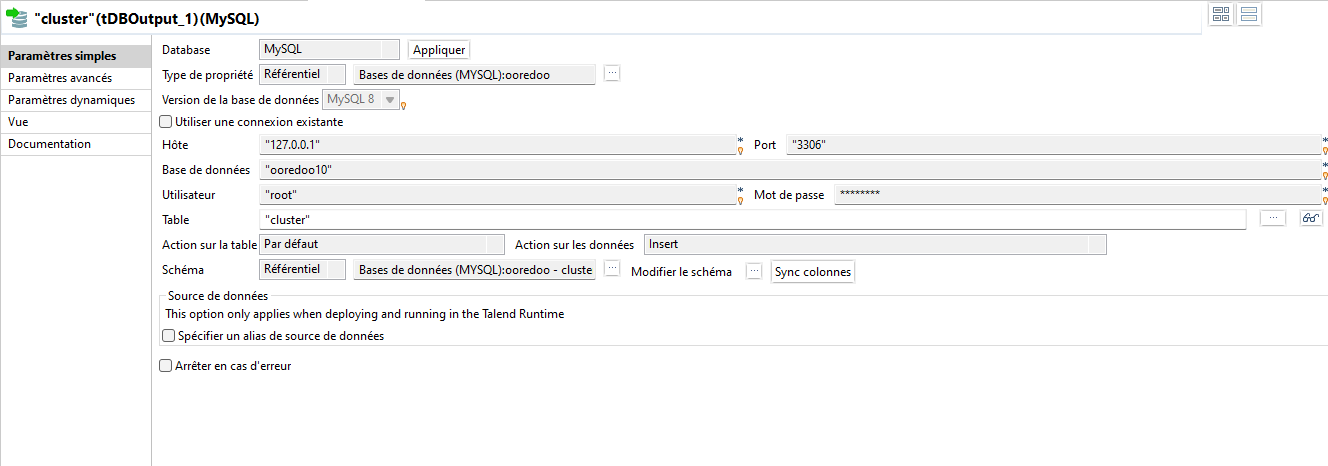
\includegraphics[width=0.8\textwidth,height=0.4\textwidth]{figures/chap4 fig/etl_step5_tdboutput.png}}
          \caption{Configuration de tDBOutput}
          \label{fig:etl_step5}
      \end{figure}
\end{itemize}

\begin{figure}[h]
    \centering
    \frame{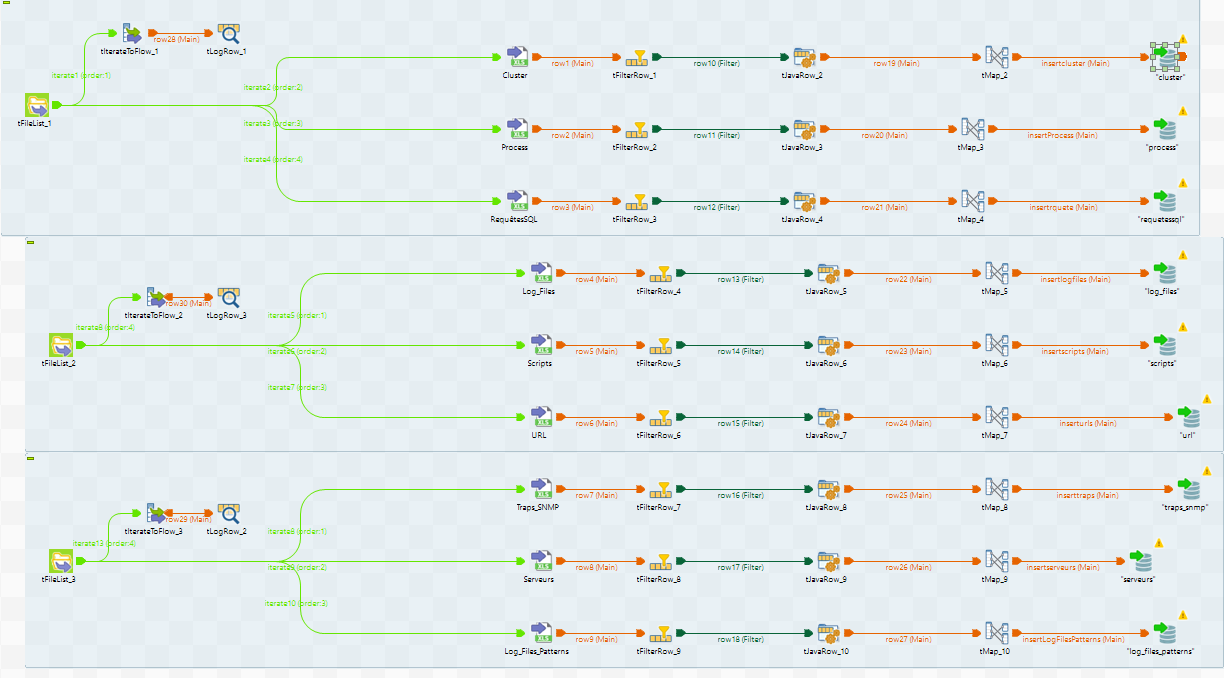
\includegraphics[width=0.8\textwidth,height=0.4\textwidth]{figures/chap4 fig/etl_workflow.png}}
    \caption{Workflow ETL avec Talend}
    \label{fig:etl_workflow}
\end{figure}

\subsection{Développement de l’API RESTful}

Dans le cadre de ce projet, j’ai entrepris la création d’une API RESTful avec Laravel pour gérer les demandes de supervision et leurs éléments associés (serveurs, URLs, processus, etc.). Ce travail a impliqué la génération des migrations, modèles, contrôleurs et routes, en m’appuyant sur les structures des tables définies précédemment. Voici comment j’ai procédé étape par étape :

\begin{itemize}
    \item \textbf{Générer les migrations et modèles pour les tables (ex. `demandes`, `users`)}  
      J’ai commencé par créer les migrations pour les tables principales et de supervision en utilisant la commande `php artisan make:migration`. Pour la table `demandes`, j’ai défini les colonnes comme `id`, `status\_id`, `user\_id`, et `serviceplatfom\_id`, avec des clés étrangères ajoutées dans une migration séparée pour assurer l’intégrité référentielle. Ensuite, j’ai généré les modèles avec `php artisan make:model`, en utilisant l’outil Reliese pour automatiser la création de relations (ex. `hasMany` pour les tables de supervision comme `urls` ou `processes`). Une capture montre un exemple de migration que j’ai configurée pour la table `demandes`.
      
      \begin{figure}[h]
          \centering
          \frame{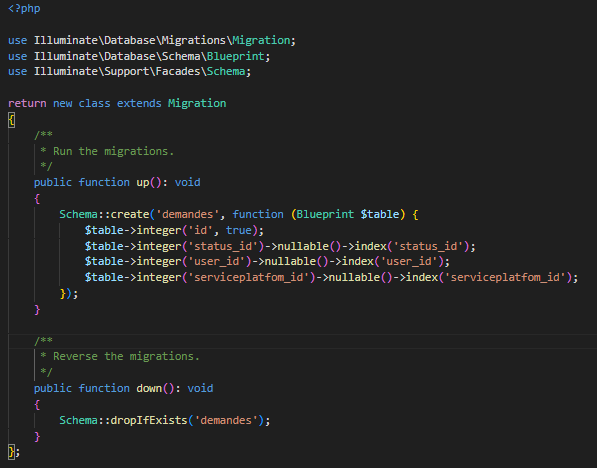
\includegraphics[width=0.8\textwidth,height=0.4\textwidth]{figures/chap4 fig/migration_demandes.png}}
          \caption{Exemple de migration pour la table `demandes`}
          \label{fig:migration_demandes}
      \end{figure}
      
    \item \textbf{Développer les contrôleurs pour gérer les endpoints CRUD}  
      J’ai créé le contrôleur `DemandeController` avec `php artisan make:controller DemandeController --api` pour implémenter les méthodes CRUD (index, store, show, update, destroy). J’ai ajouté des validations dans la méthode `store` pour s’assurer que les champs comme `description` et `status\_id` respectent les contraintes, et j’ai intégré une logique pour générer une référence unique (`ref`) basée sur la date et le nom de la plateforme. Pour la méthode `show`, j’ai utilisé `with()` pour charger les relations (ex. `serveurs`, `urls`), optimisant ainsi les performances. Une capture illustre une partie du code du contrôleur que j’ai développé.
      
      \begin{figure}[h]
          \centering
          \frame{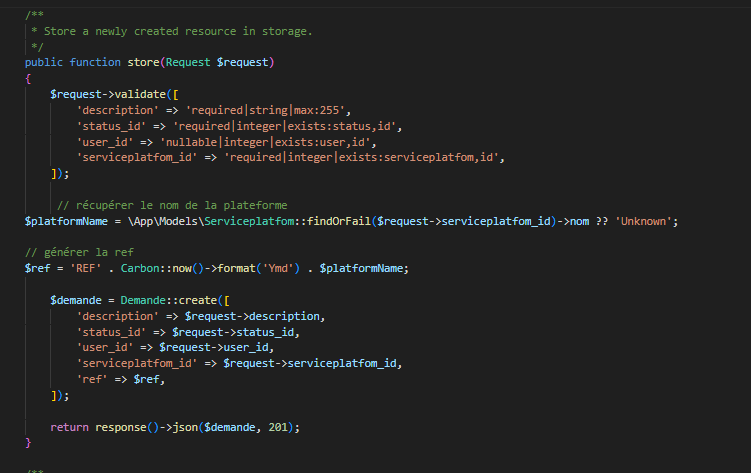
\includegraphics[width=0.8\textwidth,height=0.4\textwidth]{figures/chap4 fig/controller_demandes.png}}
          \caption{Exemple de méthode dans le contrôleur `DemandeController`}
          \label{fig:controller_demandes}
      \end{figure}
      
    \item \textbf{Définir les routes dans `routes/api.php` (ex. `/demandes`, `/demandes/{id}`)}  
      J’ai configuré les routes dans `routes/api.php` en utilisant `Route::apiResource` pour automatiser la création des endpoints CRUD pour toutes les tables (ex. `demandes`, `serveurs`, `urls`). J’ai également ajouté un groupe de middleware `auth:sanctum` pour sécuriser les routes après authentification LDAP via `/login`. Cela m’a permis de gérer les permissions et de protéger les données sensibles. Une capture montre une partie de la configuration des routes que j’ai mise en place.
      
      \begin{figure}[h]
          \centering
          \frame{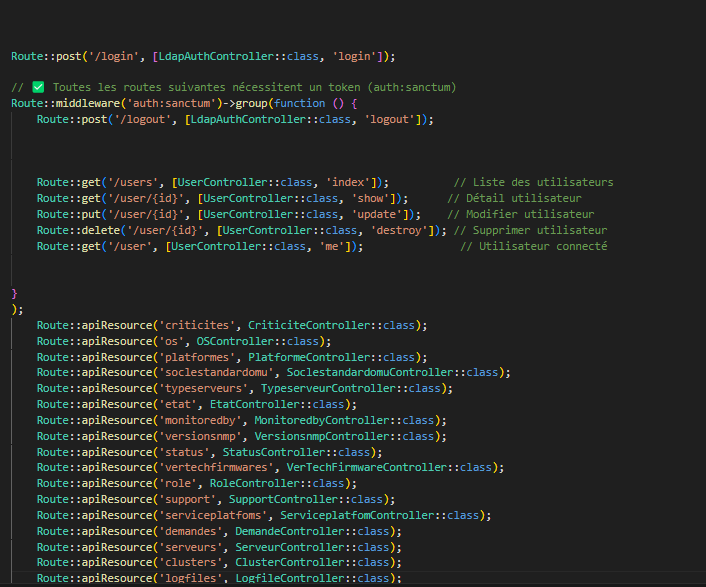
\includegraphics[width=0.8\textwidth,height=0.4\textwidth]{figures/chap4 fig/routes_api.png}}
          \caption{Exemple de configuration des routes dans `routes/api.php`}
          \label{fig:routes_api}
      \end{figure}
\end{itemize}

Mon travail sur l’API a été guidé par l’objectif de fournir une interface robuste et scalable. J’ai testé chaque endpoint avec Postman pour valider les réponses JSON et j’ai utilisé les relations Eloquent pour lier les tables de supervision aux demandes, facilitant ainsi la récupération des données associées. Les captures fournies reflètent les parties clés de mon code, illustrant mon approche pratique dans ce projet.

\subsection{Intégration de l’authentification LDAP}

Dans le cadre de ce projet, j’ai intégré une authentification LDAP avec Laravel pour sécuriser l’accès à l’API RESTful, en utilisant un serveur LDAP externe (ex. forumsys.com) comme modèle. Cette étape a été essentielle pour connecter les utilisateurs aux rôles et supports définis dans la base de données. Voici comment j’ai configuré et implémenté cette fonctionnalité étape par étape :

\begin{itemize}
    \item \textbf{Installer : `composer require directorytree/ldaprecord-laravel`}  
      J’ai commencé par installer le package `ldaprecord-laravel` avec la commande `composer require directorytree/ldaprecord-laravel`. Après l’installation, j’ai publié les fichiers de configuration avec `php artisan ldap:publish`, ce qui a généré le fichier `config/ldap.php`. Cette étape m’a permis de poser les bases pour la connexion au serveur LDAP. Une capture montre la configuration initiale de `.env` où j’ai défini les paramètres LDAP.
      
      \begin{figure}[h]
          \centering
          \frame{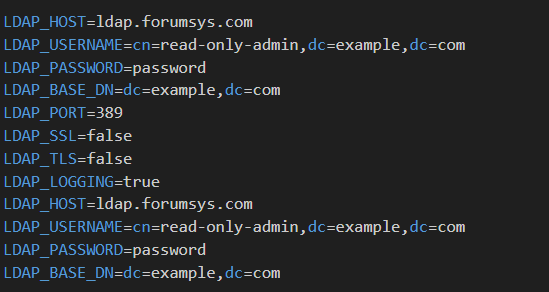
\includegraphics[width=0.8\textwidth,height=0.4\textwidth]{figures/chap4 fig/ldap_env_config.png}}
          \caption{Configuration des variables d’environnement dans `.env`}
          \label{fig:ldap_env_config}
      \end{figure}
      
    \item \textbf{Configurer `config/ldap.php` avec les paramètres LDAP}  
      J’ai personnalisé le fichier `config/ldap.php` pour spécifier les paramètres de connexion, tels que `hosts`, `username`, `password`, `base\_dn`, et `port`. J’ai utilisé des variables d’environnement (`env()`) pour rendre la configuration flexible et sécurisée. J’ai désactivé `use\_ssl` et `use\_tls` pour ce serveur test, tout en activant le logging pour déboguer les erreurs. Une capture illustre une partie de la configuration que j’ai mise en place.
      
      \begin{figure}[h]
          \centering
          \frame{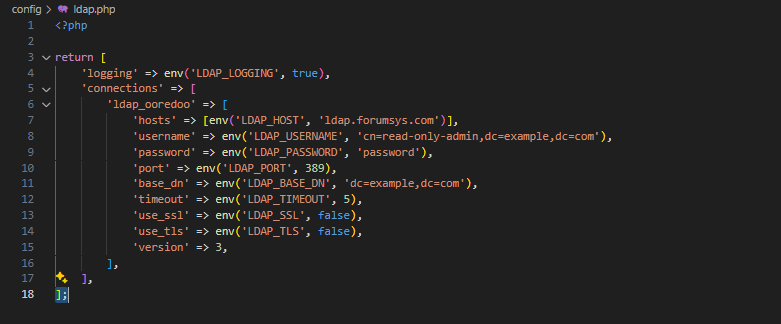
\includegraphics[width=0.8\textwidth,height=0.4\textwidth]{figures/chap4 fig/ldap_config_file.png}}
          \caption{Extrait de la configuration dans `config/ldap.php`}
          \label{fig:ldap_config_file}
      \end{figure}
      
    \item \textbf{Configurer Sanctum pour les tokens}  
      J’ai installé Laravel Sanctum avec `composer require laravel/sanctum` et configuré les domaines autorisés dans `.env` (ex. `localhost:3000`). J’ai ensuite exécuté `php artisan vendor:publish --provider="Laravel\Sanctum\SanctumServiceProvider"` pour publier les configurations. Cela m’a permis de générer des jetons d’accès après une authentification réussie, sécurisant les endpoints de l’API. Une capture montre une partie de la configuration Sanctum dans `.env`.
      
      \begin{figure}[h]
          \centering
          \frame{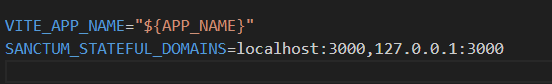
\includegraphics[width=0.6\textwidth,height=0.1\textwidth]{figures/chap4 fig/sanctum_env_config.png}}
          \caption{Configuration Sanctum dans `.env`}
          \label{fig:sanctum_env_config}
      \end{figure}
      
    \item \textbf{Mettre à jour `config/auth.php` pour utiliser LDAP}  
      J’ai modifié `config/auth.php` pour intégrer LDAP comme fournisseur d’authentification. Cependant, comme le package LDAP ne remplace pas totalement Eloquent, j’ai conservé le driver `eloquent` pour la gestion des utilisateurs locaux, en synchronisant les données LDAP avec la table `users`. Une capture illustre la section pertinente de `config/auth.php` que j’ai ajustée.
      
      \begin{figure}[h]
          \centering
          \frame{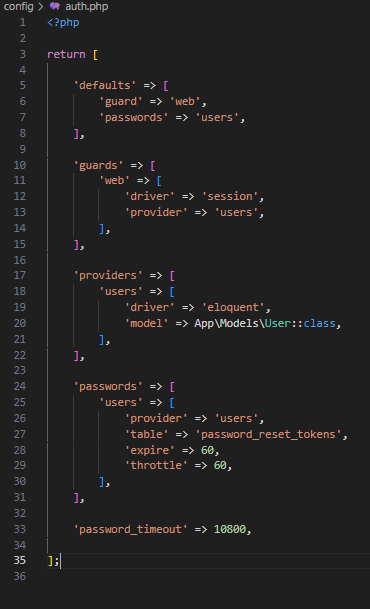
\includegraphics[width=0.4\textwidth]{figures/chap4 fig/auth_config_file.png}}
          \caption{Extrait de la configuration dans `config/auth.php`}
          \label{fig:auth_config_file}
      \end{figure}
      
    \item \textbf{Créer un `AuthController` pour gérer la logique d’authentification}  
      J’ai créé le contrôleur `LdapAuthController` avec `php artisan make:controller Auth/LdapAuthController` pour gérer la logique de connexion et de déconnexion. J’ai implémenté la méthode `login` pour valider les identifiants, tenter une authentification LDAP, et créer ou mettre à jour un utilisateur local avec son rôle basé sur les groupes LDAP (ex. "scientists" pour admin). La méthode `logout` supprime les jetons. Une capture montre une partie du code du contrôleur que j’ai développé.
      
      \begin{figure}[h]
          \centering
          \frame{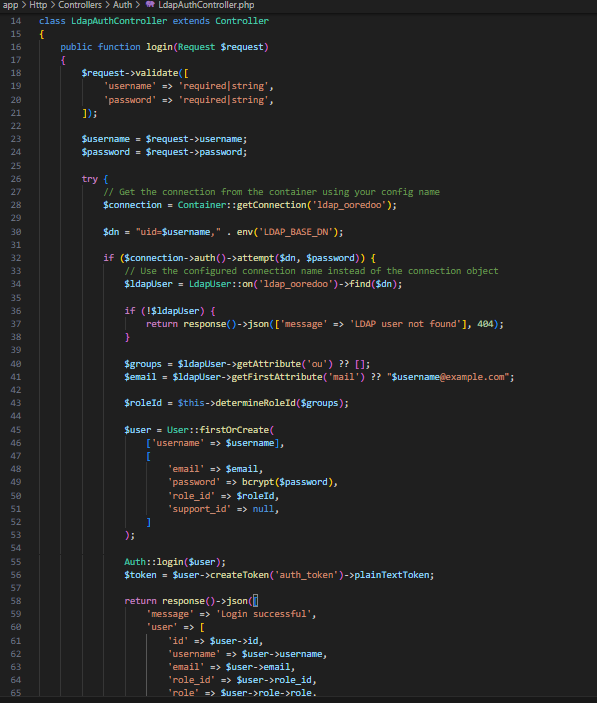
\includegraphics[width=0.8\textwidth,height=0.4\textwidth]{figures/chap4 fig/ldap_auth_controller.png}}
          \caption{Extrait de la méthode `login` dans `LdapAuthController`}
          \label{fig:ldap_auth_controller}
      \end{figure}
\end{itemize}

J’ai testé l’authentification avec Postman en envoyant une requête POST à `/login` avec des identifiants valides, vérifiant la réponse JSON contenant le jeton et les informations utilisateur. Cette intégration m’a permis de sécuriser l’API tout en synchronisant les utilisateurs LDAP avec la base de données locale, un point clé pour la gestion des permissions dans le projet.

\subsection{Interface de soumission des demandes}

Dans le cadre de ce projet, j’ai développé l’interface de soumission des demandes avec Nuxt.js, en m’appuyant sur un design modulaire et interactif pour répondre aux besoins des utilisateurs. J’ai opté pour un formulaire présenté sous forme de modal, inspiré de l’interface du tableau de bord fournie, afin de centraliser la création des demandes et leur association avec les tables EBDS (ex. Serveurs, URLs, Processus) dans une expérience utilisateur fluide. Voici comment j’ai conçu et implémenté cette interface :

\begin{itemize}
    \item \textbf{Conception du modal principal pour la demande}  
      J’ai créé un modal accessible via le bouton "Ajouter Demande" sur le tableau de bord. Ce modal débute par un formulaire de base pour la demande, incluant des champs comme `description`, `plateforme de service` (sélectionnée via une liste déroulante), et un bouton "Créer la demande" pour soumettre les données à l’API RESTful via une requête POST à `/demandes`. Une fois la demande créée, un identifiant unique (`ref`) est généré et affiché. Une capture montre l’interface initiale du modal que j’ai développée.
      
      \begin{figure}[h]
          \centering
          \frame{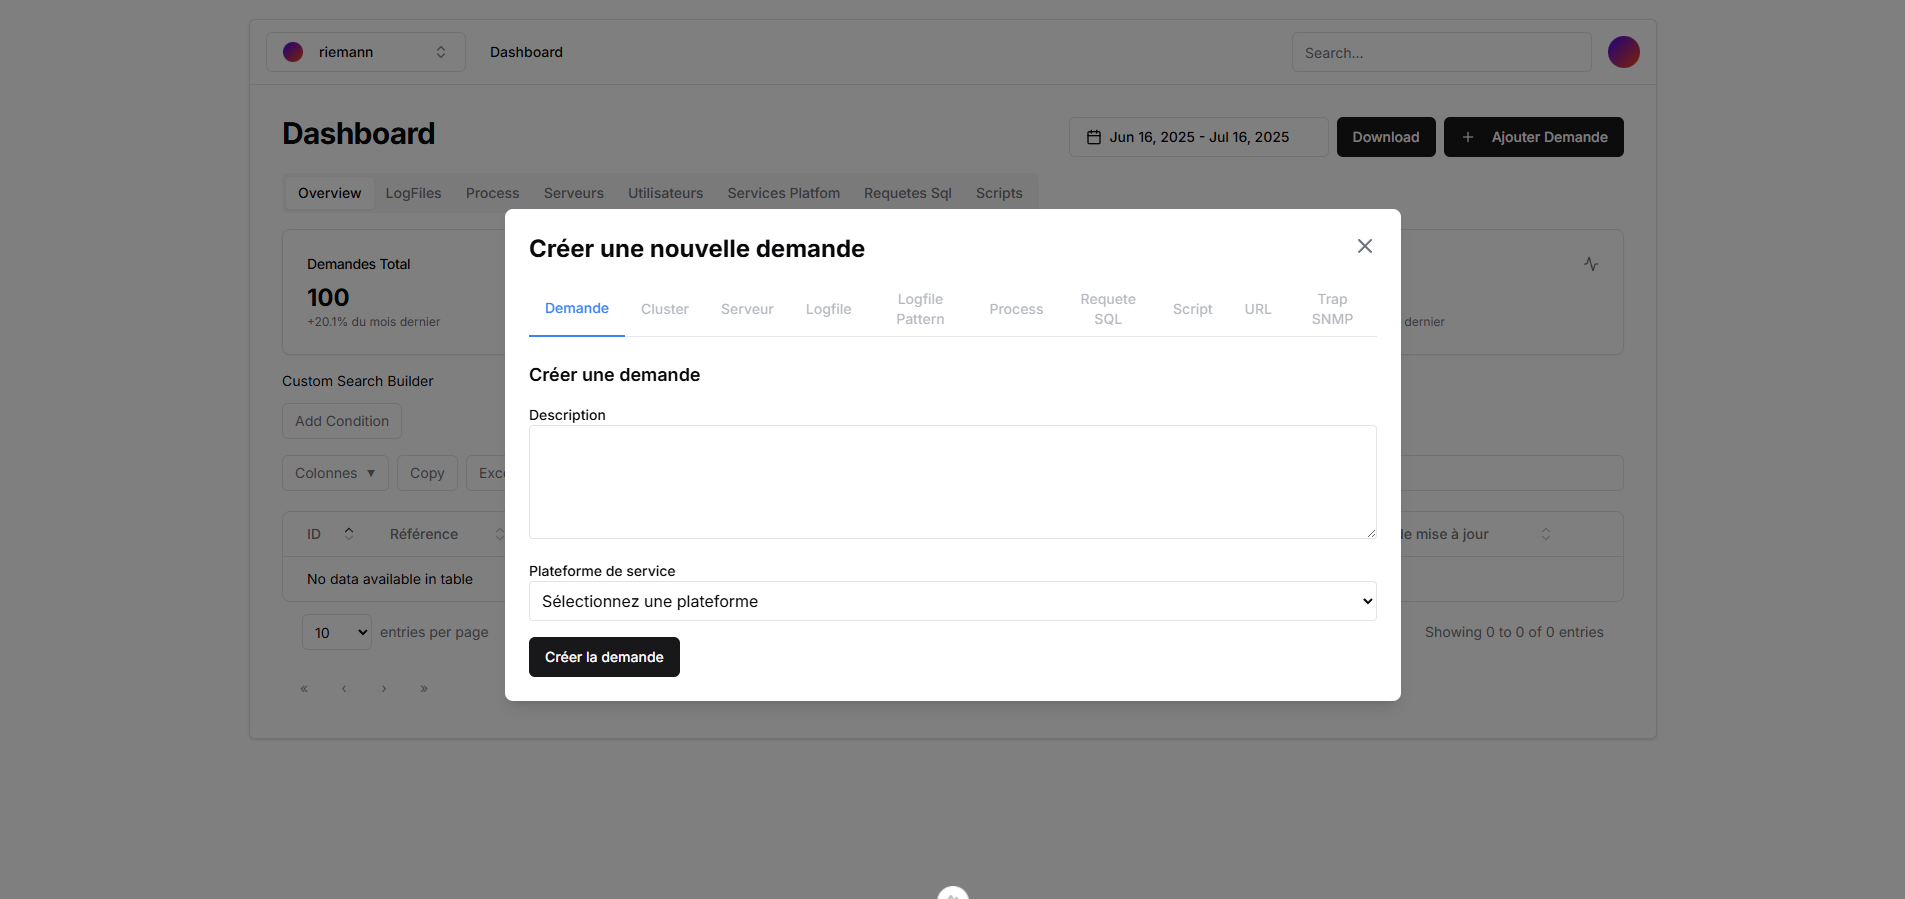
\includegraphics[width=0.8\textwidth,height=0.4\textwidth]{figures/chap4 fig/submission_ui.png}}
          \caption{Interface de soumission des demandes (étape initiale)}
          \label{fig:submission_ui_initial}
      \end{figure}
      
    \item \textbf{Gestion des tables associées en plusieurs étapes}  
      Après la création de la demande, j’ai ajouté une section dans le même modal pour gérer les tables associées (ex. Serveurs, URLs). Cette section s’active via un onglet ou un bouton "Ajouter éléments associés", permettant d’afficher un sous-formulaire dynamique. J’ai implémenté une interface en plusieurs étapes :  
      - **Ajout** : Un menu déroulant permet de sélectionner le type d’élément (Cluster, Serveur, Logfile, etc.), suivi d’un formulaire spécifique pour entrer les détails (ex. `hostname` pour Serveur, `url` pour URL).  
      - **Affichage** : Une liste des éléments associés s’affiche dans le modal, avec des détails comme `id` et `description`.  
      - **Modification/Suppression** : Chaque élément inclut des boutons pour éditer (via un formulaire pop-up dans le modal) ou supprimer (via une confirmation). Ces actions sont synchronisées avec l’API via des endpoints comme `/serveurs/{id}` ou `/urls/{id}`.
      
      \begin{figure}[h]
          \centering
          \frame{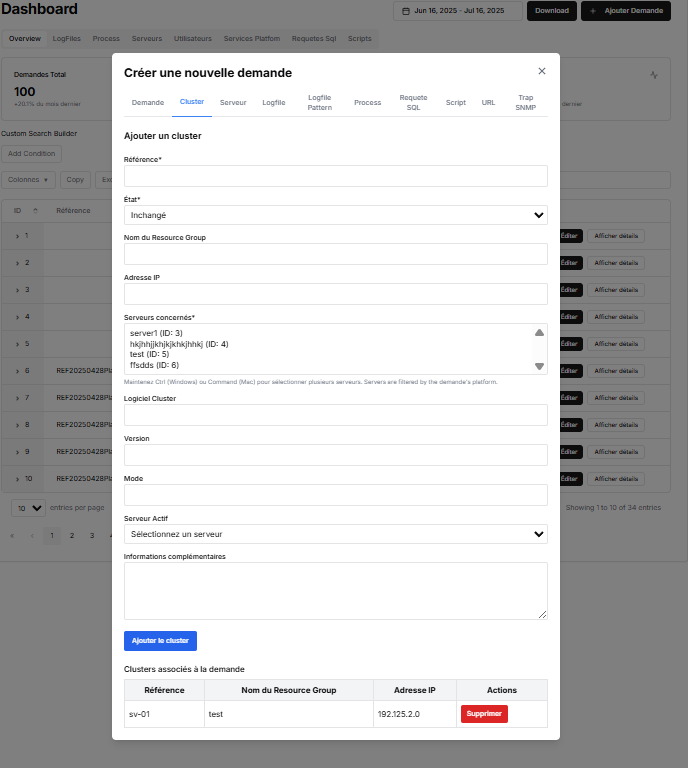
\includegraphics[width=0.8\textwidth,height=0.6\textwidth]{figures/chap4 fig/submission_ui_associated.png}}
          \caption{Interface de soumission avec gestion des tables associées}
          \label{fig:submission_ui_associated}
      \end{figure}
      
    \item \textbf{Interaction et validation}  
      J’ai intégré des validations côté client avec VeeValidate pour vérifier les champs avant soumission (ex. `plateforme de service` obligatoire). Une fois tous les éléments associés validés, un bouton final "Enregistrer tout" envoie les données à l’API, mettant à jour la demande et ses relations. J’ai testé cette interface avec des données fictives pour assurer une navigation fluide entre les étapes. Une capture montre l’état final du modal après ajout et validation.
\end{itemize}

Cette approche m’a permis de créer une interface intuitive et fonctionnelle. Le modal centralise toutes les actions, réduisant les allers-retours entre différentes vues, et s’aligne avec les exigences du projet pour gérer les données complexes des tables EBDS. Les captures reflètent les différentes étapes de mon développement, illustrant l’évolution de l’interface.

\subsection{Interface de gestion des demandes}

Dans le cadre de ce projet, j’ai développé une interface administrateur avec Nuxt.js pour gérer les demandes, en mettant l’accent sur une fonctionnalité de filtrage avancée implémentée en JavaScript. j’ai conçu un système interactif pour filtrer les demandes de manière personnalisée, en me basant sur les données de la base via l’API RESTful. Voici comment j’ai procédé :

J’ai intégré un panneau de filtrage dynamique, accessible via un "Custom Search Builder", où les administrateurs peuvent sélectionner des colonnes spécifiques à filtrer. J’ai listé les colonnes disponibles, comme `État`, `Adresse IP`, `Nom RPGS`, ou `Référence`, en les récupérant dynamiquement depuis les en-têtes des tables (ex. `status`, `serveurs`). L’utilisateur choisit une colonne via une liste déroulante. Ensuite, j’ai ajouté un sélecteur d’opérateurs, offrant des options comme "equals" (égal à), "contains" (contient), ou même une option personnalisée "je ne sais pas" pour des cas non définis, permettant une flexibilité dans les critères. Une fois l’opérateur sélectionné, un champ de saisie permet d’entrer la valeur à filtrer (ex. "Nouveau" pour `État`, "192.168.1.1" pour `Adresse IP`).

Pour rendre le filtrage plus puissant, j’ai implémenté la possibilité d’ajouter d’autres conditions. Un bouton "Add Condition" génère une nouvelle ligne de filtrage, où l’utilisateur peut choisir une autre colonne et un autre opérateur, puis entrer une nouvelle valeur. J’ai ajouté une logique pour combiner ces conditions avec des opérateurs logiques : un menu déroulant permet de sélectionner "OR" (ou) ou "AND" (et) entre les conditions. Par exemple, on peut filtrer les demandes où `État` equals "Nouveau" AND `Adresse IP` contains "192.168.1", ou encore `État` equals "Clôturée" OR `Nom RPGS` contains "RPGS-01". J’ai testé cette fonctionnalité avec des données fictives pour valider la combinaison des filtres, en m’assurant que les requêtes envoyées à l’API reflètent correctement les critères sélectionnés.

\begin{figure}[h]
    \centering
    \frame{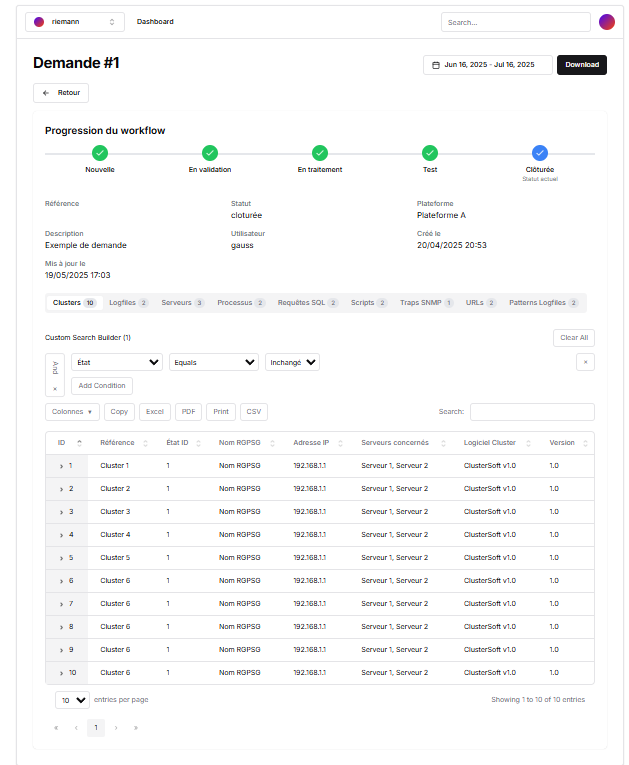
\includegraphics[width=0.8\textwidth,height=0.6\textwidth]{figures/chap4 fig/management_ui.png}}
    \caption{Interface de gestion des demandes)}
    \label{fig:management_ui_filters}
\end{figure}

\subsection{Interface de conversation}

Dans le cadre de ce projet, j’ai développé une interface de chat avec Nuxt.js pour faciliter les interactions entre les utilisateurs (demandeurs) et les administrateurs, en m’inspirant de l’exemple de conversation fourni pour la demande #1. Aujourd’hui, le 17/06/2025 à 11:21 AM CET, j’ai conçu cette fonctionnalité pour améliorer la communication autour des demandes, en intégrant un système de messagerie connecté à l’API RESTful. Voici comment j’ai implémenté cette interface :

\begin{itemize}
    \item \textbf{Intégration du bouton de conversation}  
      J’ai ajouté un bouton "Ouvrir la conversation" à côté de chaque espace de gestion de demande dans l’interface administrateur, visible dans le tableau de bord ou la vue détaillée d’une demande (ex. demande #1). Ce bouton déclenche l’ouverture d’un modal de chat, comme illustré dans la capture. J’ai assuré que ce bouton soit uniquement accessible aux utilisateurs ayant le rôle d’admin, vérifié via l’authentification Sanctum et la table `roles`. Une capture montre l’interface de chat que j’ai développée.
      
      \begin{figure}[h]
          \centering
          \frame{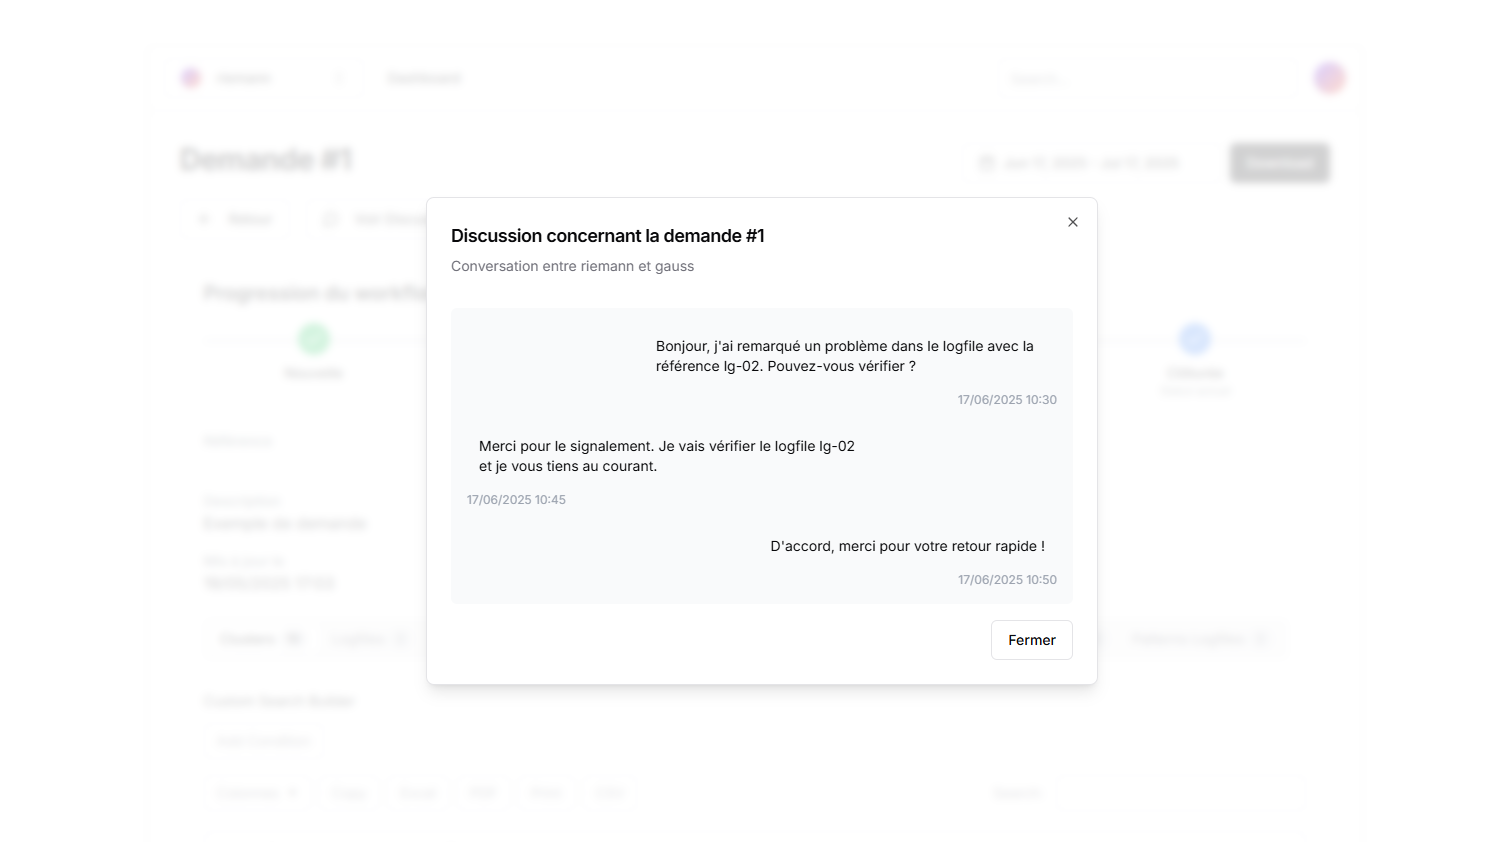
\includegraphics[width=0.8\textwidth,height=0.4\textwidth]{figures/chap4 fig/chat_ui.png}}
          \caption{Interface de conversation}
          \label{fig:chat_ui}
      \end{figure}
      
    \item \textbf{Restriction à l’admin et message direct}  
      J’ai implémenté une logique pour limiter l’ouverture de la conversation aux administrateurs uniquement. Lorsque l’admin clique sur le bouton, un modal s’affiche avec l’historique des messages (ex. entre "riemann" et "gauss" pour la demande #1) et un champ pour envoyer un nouveau message. Le message est envoyé directement au demandeur associé à la demande (ex. "gauss") via une requête POST à un endpoint personnalisé comme `/demandes/{id}/messages`. J’ai utilisé WebSockets ou des appels API en temps réel pour notifier le demandeur immédiatement. La capture montre un exemple de conversation initiée par l’admin.
      
    \item \textbf{Gestion de l’interaction}  
      J’ai conçu le chat pour afficher les messages avec les noms des participants et les horodatages (ex. 17/06/2025 10:45), permettant à l’admin de suivre la discussion. Le demandeur ne peut pas initier la conversation mais peut répondre une fois qu’elle est ouverte. J’ai ajouté un bouton "Fermer" pour terminer la session de chat. J’ai testé cette fonctionnalité avec des utilisateurs fictifs pour valider la fluidité de l’échange et la sécurité des permissions.
\end{itemize}

Cette interface m’a permis de créer un canal de communication efficace et sécurisé. Le bouton d’ouverture, réservé aux admins, garantit une gestion contrôlée des interactions, tandis que la messagerie directe améliore la résolution des problèmes signalés, comme illustré dans l’exemple de la demande #1.

\section{Réalisation du tableau de bord}

\subsection{Connexion à la base de données}

Connexion de Power BI à MySQL pour extraire les données agrégées.

\begin{figure}[h]
    \centering
    \frame{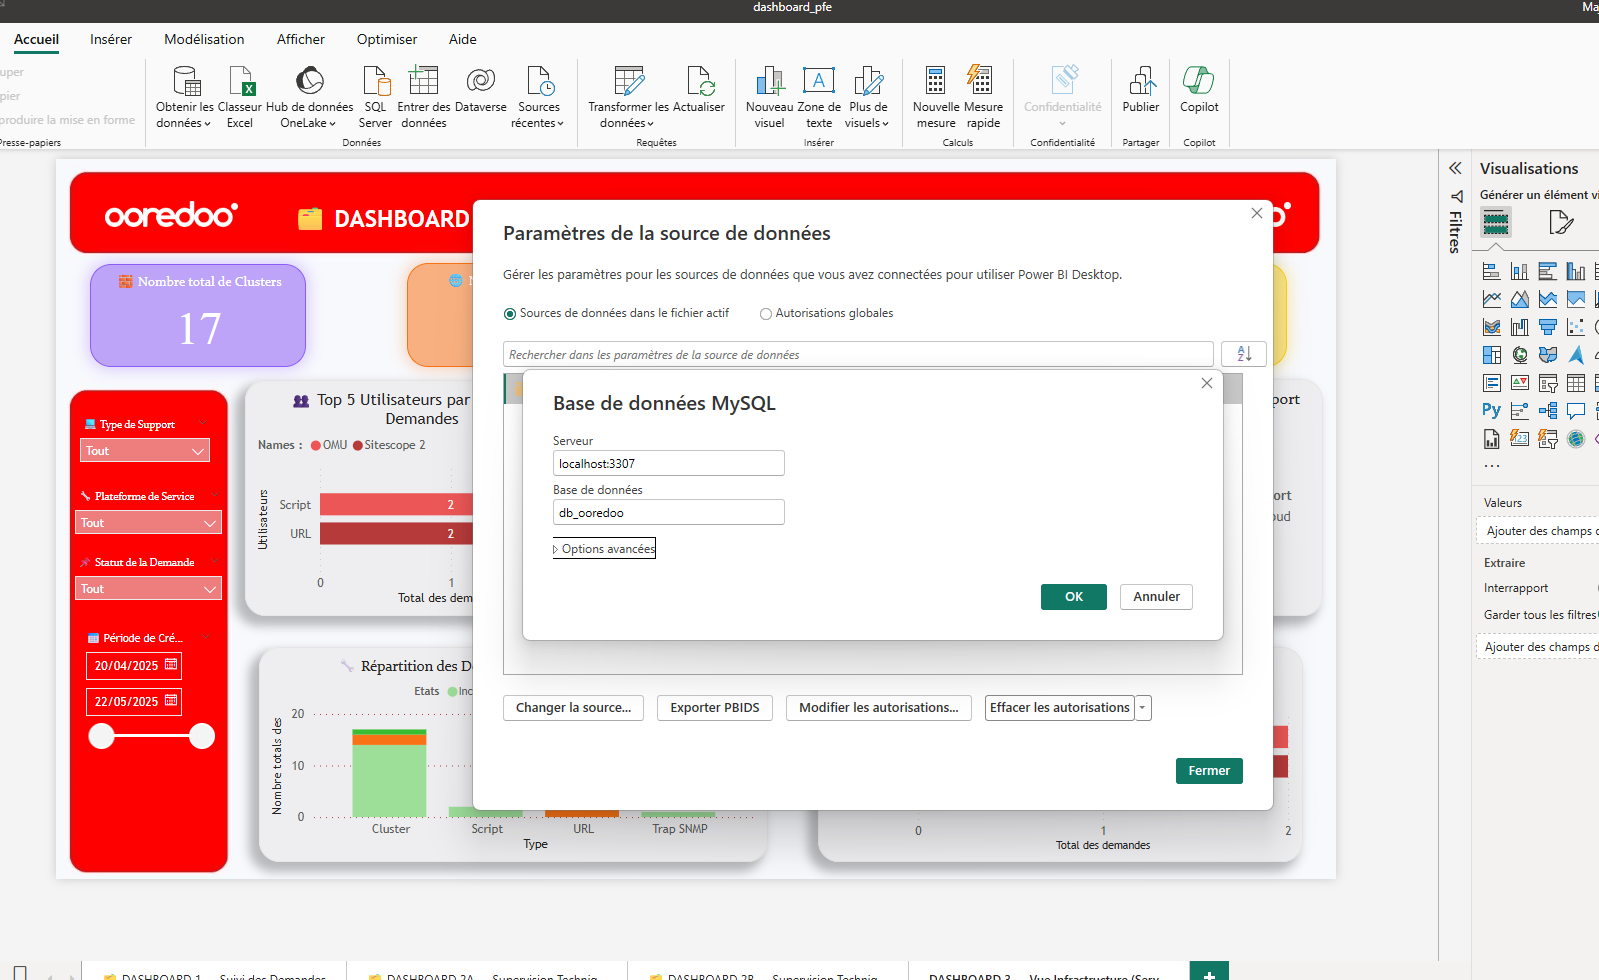
\includegraphics[width=0.8\textwidth,height=0.4\textwidth]{figures/chap4 fig/powerbi_connection.png}}
    \caption{Connexion Power BI à MySQL}
    \label{fig:powerbi_connection}
\end{figure}

\subsection{Réalisation des tableaux de bord}

Quatre tableaux de bord créés avec Power BI :

\begin{itemize}
    \item \textbf{DASHBOARD 1 — Suivi des Demandes} : Suivi de l’évolution et de la répartition des demandes.
    \item \textbf{DASHBOARD 2A — Supervision Technique : Composants Techniques} : Visualisation des composants techniques par demande.
    \item \textbf{DASHBOARD 2B — Supervision Technique : Supervision Applicative} : Suivi des éléments applicatifs.
    \item \textbf{DASHBOARD 3 — Vue Infrastructure} : Répartition des ressources (serveurs, plateformes).
\end{itemize}

\begin{figure}[h]
    \centering
    \frame{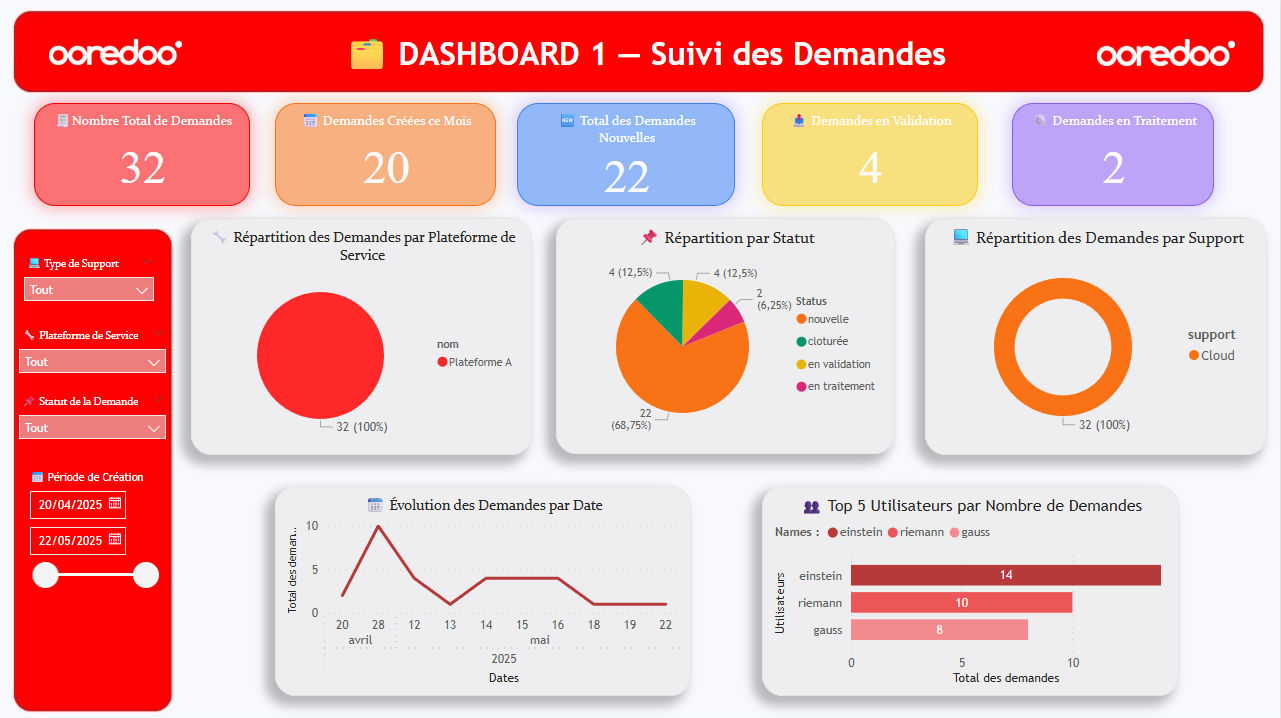
\includegraphics[width=0.8\textwidth,height=0.4\textwidth]{figures/chap4 fig/dashboard1.png}}
    \caption{Dashboard 1 : Suivi des Demandes}
    \label{fig:dashboard1}
\end{figure}

\begin{figure}[h]
    \centering
    \frame{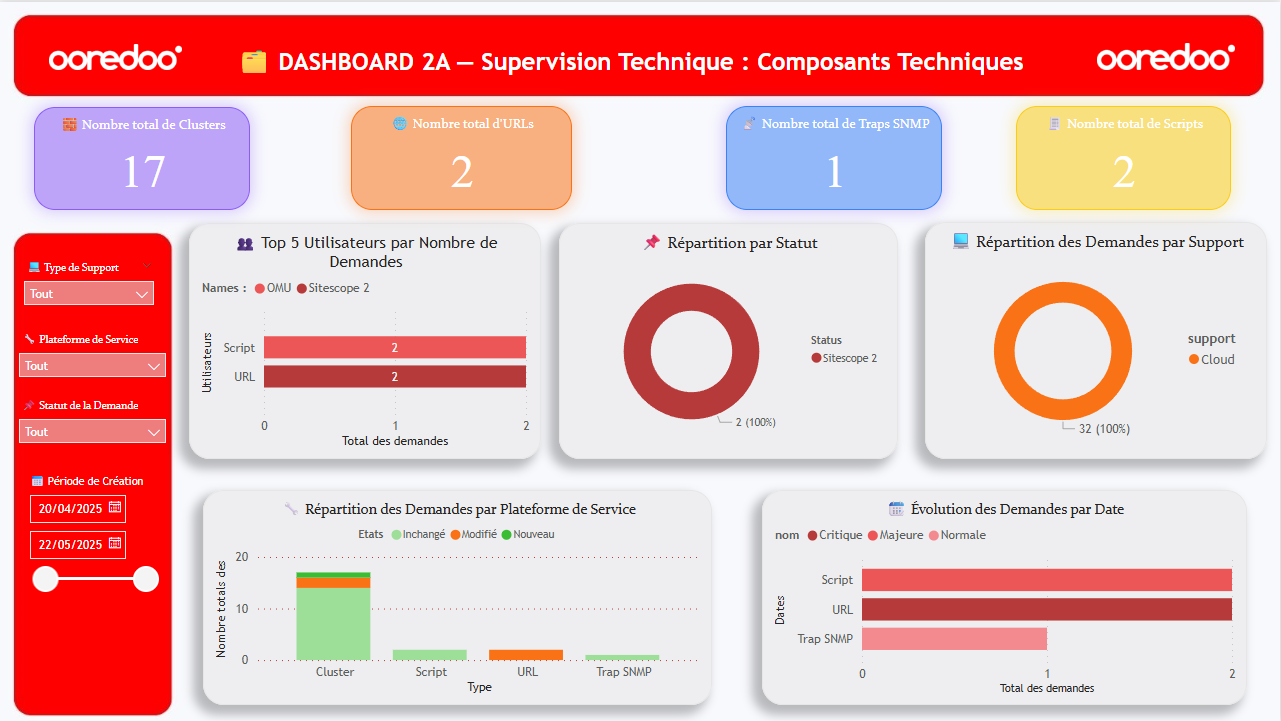
\includegraphics[width=0.8\textwidth,height=0.4\textwidth]{figures/chap4 fig/dashboard2a.png}}
    \caption{Dashboard 2A : Supervision Technique (Composants)}
    \label{fig:dashboard2a}
\end{figure}

\begin{figure}[h]
    \centering
    \frame{\includegraphics[width=0.8\textwidth,height=0.4\textwidth]{figures/chap4 fig/dashboard2b.png}}
    \caption{Dashboard 2B : Supervision Technique (Applicative)}
    \label{fig:dashboard2b}
\end{figure}

\begin{figure}[h]
    \centering
    \frame{\includegraphics[width=0.8\textwidth,height=0.4\textwidth]{figures/chap4 fig/dashboard3.png}}
    \caption{Dashboard 3 : Vue Infrastructure}
    \label{fig:dashboard3}
\end{figure}

\section{Réalisation du chatbot}

Chatbot développé avec Ollama et Python, répondant à des questions via des requêtes SQL.

\begin{itemize}
    \item Génère des requêtes SQL (ex. `SELECT COUNT(*) FROM demandes WHERE date_creation = CURDATE();`).
    \item Déployé avec une API Flask et intégré au frontend Nuxt.js.
\end{itemize}

\begin{figure}[h]
    \centering
    \frame{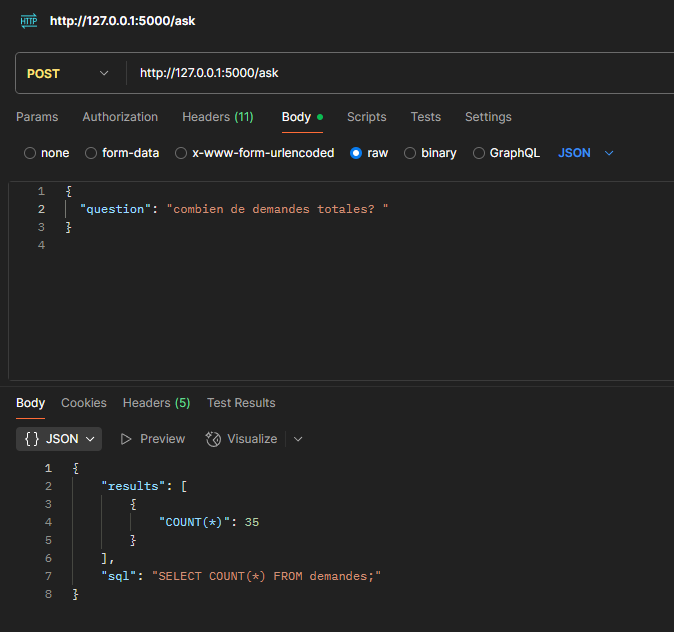
\includegraphics[width=0.8\textwidth,height=0.4\textwidth]{figures/chap4 fig/postman_response.png}}
    \caption{Réponse Postman du chatbot}
    \label{fig:postman_response}
\end{figure}

\begin{figure}[h]
    \centering
    \frame{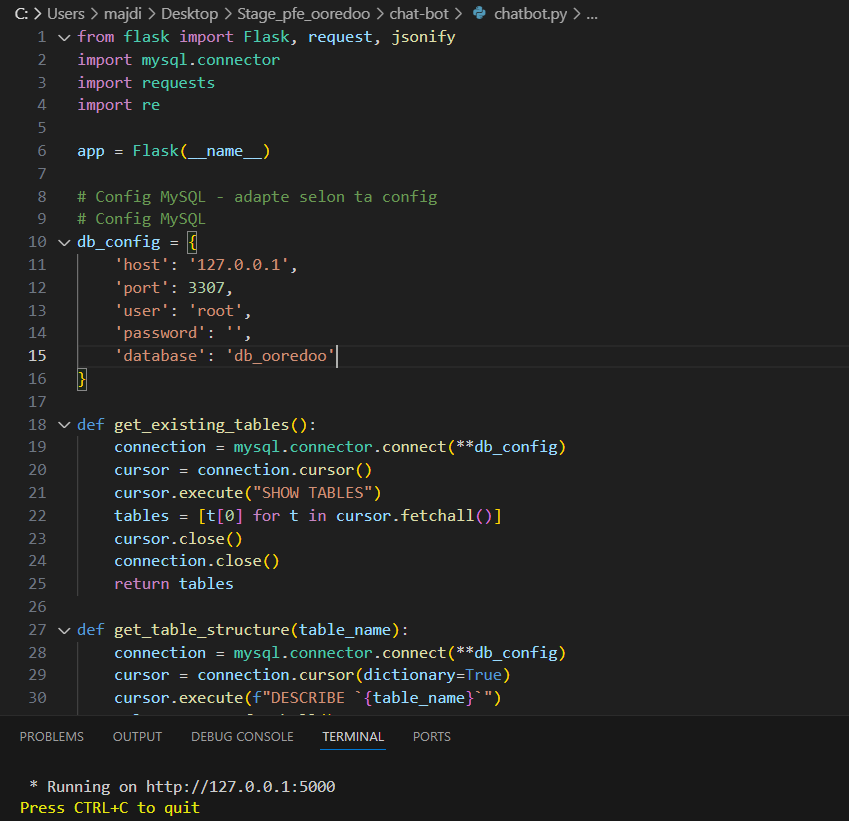
\includegraphics[width=0.8\textwidth,height=0.4\textwidth]{figures/chap4 fig/chat_flask.png}}
    \caption{Déploiement Flask du chatbot}
    \label{fig:chat_flask}
\end{figure}

\section{Déploiement et tests}

\subsection{Tests d’intégration}

Vérification de l’intégration entre backend, frontend, et bases de données.

\begin{figure}[h]
    \centering
    \frame{\includegraphics[width=0.8\textwidth,height=0.4\textwidth]{figures/chap4 fig/integration_test.png}}
    \caption{Exemple de test d’intégration}
    \label{fig:integration_test}
\end{figure}

\subsection{Déploiement en production}

Déploiement de l’application sur un serveur avec Laravel, Nuxt.js, et Talend.

\begin{figure}[h]
    \centering
    \frame{\includegraphics[width=0.8\textwidth,height=0.4\textwidth]{figures/chap4 fig/deployment.png}}
    \caption{Configuration de déploiement}
    \label{fig:deployment}
\end{figure}

\section*{Conclusion}
Au cours de ce chapitre, nous avons présenté en détail la mise en œuvre pratique de la conception théorique de l’application. Nous avons décrit les environnements matériels et logiciels utilisés, élaboré les étapes du processus ETL, développé le backend avec une API RESTful et l’authentification LDAP, réalisé le frontend avec Nuxt.js, créé les tableaux de bord avec Power BI, développé un chatbot avec Ollama et Python, et finalisé le déploiement avec des tests et optimisations. Ces étapes permettent de concrétiser le projet, avec un déploiement opérationnel prévu pour juillet 2025.

